%------------------------------------------------------------------------------------
%	CONFIGURATION DU DOCUMENT
%------------------------------------------------------------------------------------
\documentclass[
    %draft,
    todoNote,
    english,
    french
]{ClasseGuillaume}

\title{PortefolioTitre}
\author{Flora \textsc{Piron}}
\date{\today}

%------------------------------------------------------------------------------------
%	DEBUT DU DOCUMENT
%------------------------------------------------------------------------------------
\begin{document}

% PRE-CONTENU
\frontmatter

\geometrieWord
\begin{singlespace}
\listoftodos[TODO list]
\label{table_todos} % Cette étiquette servira de point de retour
\end{singlespace}

% PAGE DE GARDE PRINCIPALE
\geometrieLarge
\begin{titlepage}
\newcommand{\HRule}{\rule{.9\linewidth}{.6pt}} % New command to make the lines in the title page
\newcommand{\decoRule}{\rule{.8\textwidth}{.4pt}} % New command for a rule to be used under figures

\begin{center}
\vspace*{.06\textheight}
{\scshape\LARGE \href{http://www.guillaumeWinant.com}{UCLouvain}\par}\vspace{1.5cm} % University name
\textsc{\Large Bachelor Thesis}\\[0.5cm] % Thesis type

\HRule \\[0.4cm] % Horizontal line
{\huge \bfseries \thetitle\par}\vspace{0.4cm} % Thesis title
\HRule \\[1.5cm] % Horizontal line
 
\begin{minipage}[t]{0.4\textwidth}
\begin{flushleft} \large
\emph{Author:}\\
\href{http://www.guillaumeWinant.com}{\theauthor} % Author name - remove the \href bracket to remove the link
\end{flushleft}
\end{minipage}
\begin{minipage}[t]{0.4\textwidth}
\begin{flushright} \large
\emph{Supervisor:} \\
\href{http://www.jamessmith.com}{Super-viseur} % Supervisor name - remove the \href bracket to remove the link  
\end{flushright}
\end{minipage}\\[2cm]
 
\vfill

\large \textit{A thesis submitted in fulfillment of the requirements\\ for the degree of Bachelor}\\[0.3cm] % University requirement text
\textit{in the}\\[0.4cm]
\href{http://www.guillaumeWinant.com}{MonGroupe}\\
\href{http://www.guillaumeWinant.com}{MonDepartement}\\[2cm] % Research group name and department name
 
\vfill

{\large \thedate}\\[1cm] % Date
%\includegraphics{Logo} % University/department logo - uncomment to place it
 
\vfill
\end{center}
\end{titlepage}
\geometrieWord

% PROFONDEUR TABLE DES MATIERES
\setcounter{tocdepth}{2}

% TABLE DES MATIERES
\tableofcontents

%------------------------------------------------------------------------------------
%	CONTENU PRINCIPAL
%------------------------------------------------------------------------------------
\mainmatter

\geometrieLarge
\begin{titlepage}

\begin{center}
\vspace*{.06\textheight}
{\scshape\LARGE UCLouvain\par}\vspace{1.5cm} % University name
\textsc{\Large Bachelor Thesis}\\[0.5cm] % Thesis type

{\huge \bfseries Cas Diagnostique\par}\vspace{0.4cm} % Thesis title
 
\begin{minipage}[t]{0.4\textwidth}
\begin{flushleft} \large
\emph{Author:}\\
\theauthor % Author name - remove the \href bracket to remove the link
\end{flushleft}
\end{minipage}
\begin{minipage}[t]{0.4\textwidth}
\begin{flushright} \large
\emph{Supervisor:} \\
Super-viseur % Supervisor name - remove the \href bracket to remove the link  
\end{flushright}
\end{minipage}\\[3cm]
 
 
\vfill
\end{center}
\end{titlepage}
\geometrieWord

\chapter{Cas Diagnostique}
\section{Résumé du cas clinique}

\subsection{Anamnèse}

\subsubsection{Contexte socio-culturel et clinique}
Patiente de $28$ ans, est d’origine Roumaine. Elle ne parle ni français ni néerlandais ni anglais ce qui impose la présence d’une interprète lors des différentes consultations. Elle est vierge et donc G0P0. Son cycle est spontané et dure $28$ jours. La date de ses dernières règles est le $02/06/2025$.

\subsubsection{Traitement actuel}
/

\subsubsection{Antécédents médicaux et chirurgicaux}
\begin{itemize}[label=\textbullet]
    \item \underline{$2018$} : Elle a présenté un kyste fonctionnel pour lequel la patiente était inquiète au point de devoir consulter. Cet antécédent n’est pas pertinent médicalement mais permet de mieux cerner la patiente.
    
    \item \underline{Août $2020$} : Une kystectomie splénique faite en Roumanie
    
    \item \underline{Septembre $2020$} : Une infection de plaie postopératoire reprise en Belgique (UCCLE) ainsi qu’un suivi à Bruges pour récidive de kystes spléniques.
\end{itemize}

\subsubsection{Affection actuelle}
\begin{itemize}[label=\textbullet]
    \item \underline{$6$ avril $2025$} : La patiente s’est présentée aux urgences pour dysménorrhée s’aggravant depuis 4 mois. Elle traite cette douleur cyclique par de l’Ibuprofène et Dafalgan sans pour autant pouvoir reprendre ses activités quotidiennes, il s’agit donc d’un grade III de dysménorrhée. Un scanner a été effectué et a révélé un kyste ovarien. L’hypothèse émise par l’urgentiste est un endométriome. A noter qu’au scanner, il est impossible de poser un    diagnostic quant à la nature du kyste.
    
    \item \underline{$5$ mai $2025$} : Lors d’une consultation gynécologique, l’examen clinique est sans particularité. L’échographie révèle un kyste ovarien uniloculaire en cycle spontané de $74\,x\,68\,x\,53$ mm à gauche compatible avec un endométriome. Une biologie qui reprend la réserve ovarienne ainsi que le CA $125$.
    
    \item \underline{$22$ mai $2025$} : La patiente se présente à un nouveau rendez-vous en gynécologie car elle souhaite une solution chirurgicale le plus vite possible. 
\end{itemize}

\subsection{Hypothèses diagnostiques}

\geometrieLarge
\begin{sidewaystable}
\centering
\caption{Les hypothèses diagnostiques}
\label{tab:hypothesesDiagnostiques}
\begin{tabular} {|>{\raggedright\arraybackslash}p{0.1\textwidth}|>{\raggedright\arraybackslash}p{0.2\textwidth}|>{\raggedright\arraybackslash}p{0.2\textwidth}|>{\raggedright\arraybackslash}p{0.2\textwidth}|>{\raggedright\arraybackslash}p{0.2\textwidth}|}
        \toprule
        Diagnostic & Définition & Symptômes & Signes cliniques & Remarques \\
        \midrule
        \hline
        Kyste hémorragique du corps jaune & Kyste fonctionnel, dépendant du cycle menstruel. & Dysménorrhée avec douleur unilatérale lors de la phase lutéale. & \vspace{-3mm} \begin{itemize}[label=\textbullet]
            \item Palpation abdominale : sensible ;
            \item Toucher vaginale : masse annexielle palpée, mobilisation utérine douloureuse.
        \end{itemize}
        & Rupture du kyste \rightarrow \hspace{5pt} défense abdominale, signe du cri du Douglas. \\
        \hline
        Endométriome & Endomètre ectopique au niveau ovarien. & Dysménorrhée, douleurs pelviennes chroniques, dyspareunie profonde, troubles de la fertilité. & \vspace{-3mm} \begin{itemize}[label=\textbullet]
            \item Palpation abdominale : sensible ;
            \item Toucher vaginale : masse annexielle palpable, mobilisation utérine douloureuse (adhérences suspectées), cul-de-sac du Douglas sensible.
        \end{itemize}
        & Les symptômes associés à d’autres systèmes sont observés (nycturie, dyschésie, trouble du transit, \ldots). Cependant, aucune explication scientifique ne parvient à établir un lien de causalité entre les symptômes et le kyste. \\
        \hline
        Kyste dermoïde & Tératome, tumeur bénigne d'origine embryonnaire, fréquente chez les femmes entre $16$ et $55$ ans. & Asymptomatique ou légère douleur pelvienne, métrorragie, dyspareunie et symptômes liés à une compression éventuelle. & \vspace{-3mm} \begin{itemize}[label=\textbullet]
            \item Palpation abdominale : normal ;
            \item Toucher vaginale : masse annexielle peut-être palpable. 
        \end{itemize}
        & Torsion ovarienne = urgence gynécologique \rightarrow \hspace{5pt} douleur abdominale aiguë et intense.  \\
        \hline
        Kyste para-ovarien & Kyste bénin avec pour origine le mésosaplinx. & Asymptomatique ou symptômes liés à une compression éventuelle. & \vspace{-3mm} \begin{itemize}[label=\textbullet]
            \item Palpation abdominale : normal ;
            \item Toucher vaginale : masse annexielle peut-être palpable. 
        \end{itemize}
        &  \\
        \hline
        \vspace{-3mm} Tumeur ovarienne & \vspace{-3mm} Cancer ovarien malin. Facteurs favorisants : G$0$P$0$, ménarche précoce, cycle menstruel spontané, \ldots & \vspace{-3mm} \parbox{0.2\textwidth}{Stade précoce : paucisymptomatique.\\
        Stade avancé : AEG, perte de poids, fatigue, \ldots} 
        & \vspace{-3mm} \begin{itemize}[label=\textbullet]
            \item Palpation abdominale : signes de carcinose (ventre de batracien, \ldots);
            \item toucher vaginale : masse annexielle palpable voire d'autres masses selon le stade d'extension.
        \end{itemize} & \vspace{-3mm} Ce diagnostic doit être exclu vu son pronostic dramatique. \\
        \hline
        \end{tabular}
\end{sidewaystable}
\geometrieWord

%\mbox{}
Les différentes hypothèses diagnostiques sont reprises dans le~\cref{tab:hypothesesDiagnostiques} à la~\cpageref{tab:hypothesesDiagnostiques}.

A noter que les examens cliniques de ces pathologies sont peu discriminants. Le diagnostic sera posé notamment grâce aux différents examens complémentaires dont l’imagerie.

\begin{figure}[H]
    \centering
    %\hspace*{-11mm}
    \begin{tcolorbox}[colframe=mdtRed, colback=white, boxrule=6pt, arc=30pt, halign=center, width=16cm]
    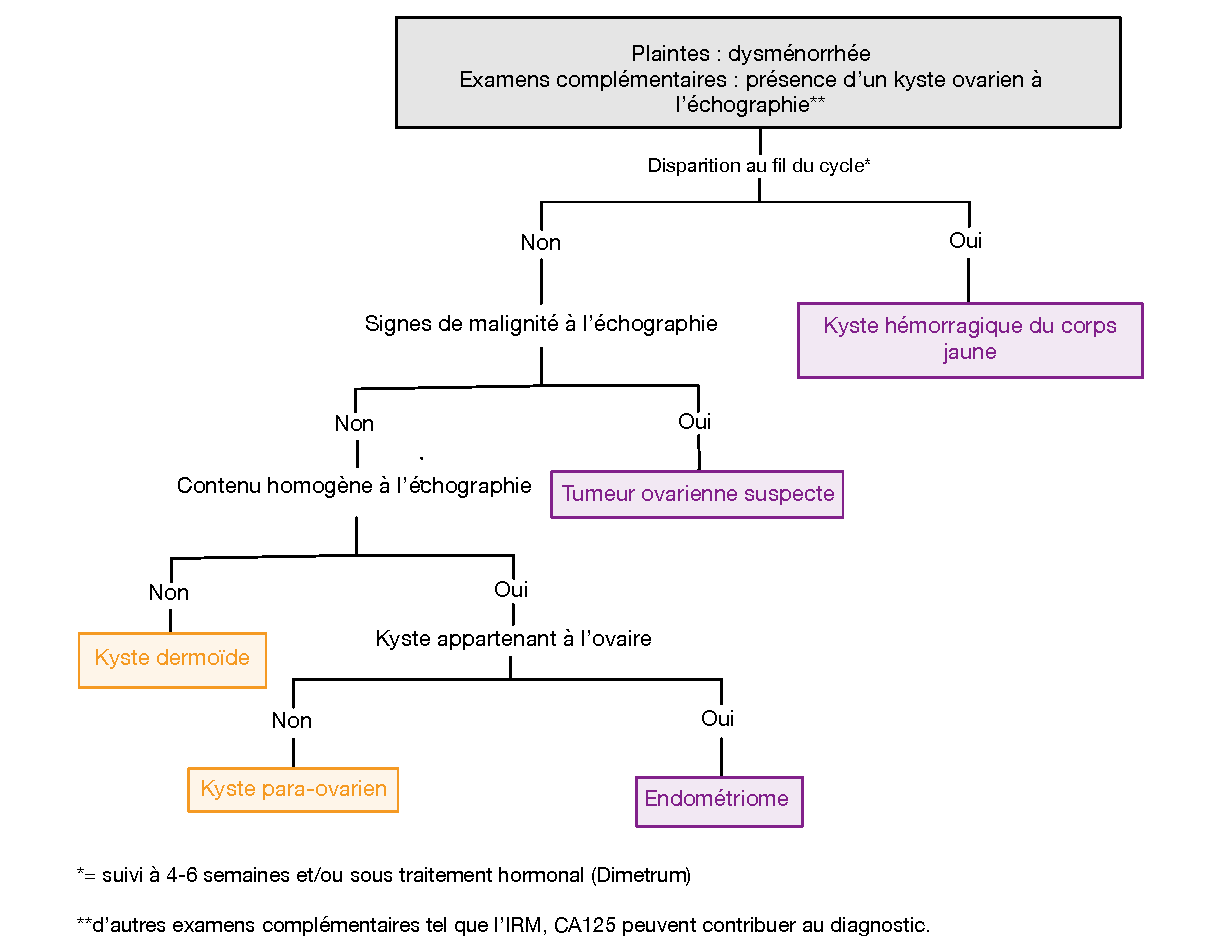
\includegraphics[width=14cm]{images/cas_diagnostique/schéma_DD.pdf}
    \end{tcolorbox}
    \caption{Arbre décisionnel des diagnostics différentiels d’un kyste ovarien chez une femme jeune en fonction de l’image échographique}
    \label{fig:ArbreDecisionMedical}
\end{figure}

\newpage

\subsection{Examen clinique} 
En gynécologie, l’examen clinique est souvent pauvre et il est nécessaire d’avoir une imagerie. Chez cette patiente, une palpation de l’abdomen a été réalisé. L’abdomen est souple, sans masse palpable. Toutefois, le toucher vaginal n’a pas été réalisé lors de la consultation car la patiente est vierge. Pourtant, un toucher vaginal pourrait donner des indications sur l’étendue de la pathologie. En effet, savoir qu’une mobilisation utérine est douloureuse ou la palpation d’autres masses éventuelles au niveau du ligament utéro-sacré, cul-de-sac de Douglas, \ldots{ } peut aider à orienter le diagnostic.

\subsection{Examens complémentaires}

\subsubsection{Biologie}
\begin{itemize}[label=\textbullet]
    \item \textbf{Justification :}\\
    une biologie a été réalisée dans le but d’évaluer le marqueur CA $125$, marqueur de l’irritation péritonéale. Son élévation est non spécifique mais présente lors d’endométriose profonde. La réserve ovarienne de la patiente est également estimé via l’AMH. Cette information aide à la prise de décision chirurgicale entre une kystectomie ou une annexectomie totale. L’hémoglobine et la coagulation sont aussi mesurées en cas de suspicion d’hémorragie intra-péritonéale et dans un contexte préopératoire proche.
    
    \item \textbf{Résultat :}%\\[0.3cm]
        \begin{table}[htbp]
\centering
\caption{Biologie - résultats}
\label{tab:examens_complementaires_resultat}
%\captionof{table}{Biologie - résultats}
\begin{tabular}{|p{0.2\textwidth}| p{0.2\textwidth}| p{0.2\textwidth}|}
    \toprule
    Nom & Quantité & Norme \\
    \midrule
    \hline
    AMH            & \SI{3.49}{\micro\gram\per\liter}         & \SIrange{1.18}{9.2}{\micro\gram\per\liter} \\
    \hline
    CA 125         & \SI{82}{\kilo\unit{U}\per\liter}         & <\SI{35}{\kilo\unit{U}\per\liter} \\
    \hline
    Hb             & \SI{13.2}{\gram\per\deci\liter}          & \SIrange{11.5}{16.5}{\gram\per\deci\liter} \\
    \hline
    PT (quick)     & \SI{92}{\percent}                        & >\SI{70}{\percent}, T25–35 \\
    \hline
    INR            & 1                                        & 1, T2.0–3.5 \\
    \hline
    aPTT           & \SI{29.8}{\second}                       & \SIrange{24.8}{34.4}{\second} \\
    \hline
    Fibrinogène    & \SI{262}{\milli\gram\per\deci\liter}     & \SIrange{200}{400}{\milli\gram\per\deci\liter} \\
    \hline
\end{tabular}
\end{table}
        %\\[1cm]
        
    \item \textbf{Impact :}\\
    L’interprétation de l’élévation de CA $125$ est complexe vu son aspécificité. Certes, lors d’endométriose profonde, le marqueur augmente mais c’est également le cas lors d’un cancer ovarien ou même lors d’un kyste fonctionnel provoquant une irritation péritonéale. Selon les autres examens, cette donnée pourra appuyer le diagnostic sans avoir un impact décisif sur celui-ci.
    
\end{itemize}

\subsubsection{Imagerie}

\begin{itemize}[label=\textbullet]
    \item \textbf{Justification :}\\
    Afin de poser le diagnostic, une échographie sera réalisée $5$ semaines après la première imagerie. Cet intervalle permet d’apprécier l’évolution du kyste. Pendant l’intervalle libre entre les deux imageries, la patiente prendra une pilule progestative, Dimetrum\textregistered dont sa principale indication thérapeutique est l’endométriose. Le Dime\-trum\textregistered\ est une pilule en continu, il induira une aménorrhée chez la patiente et inhibera l’ovulation ce qui exclura le kyste fonctionnel s’il persiste. Le Dimetrum\textregistered\ induit un environnement hypo-œstrogénique et hyperprogestogénique, ce qui entraîne une atrophie de l'endomètre eutopique et ectopique, diminuant ainsi les dysménorrhées. Un traitement hormonal joue donc un rôle diagnostic mais également thérapeutique.
    
    \item \textbf{Résultat :}\\
    Il est important de notifier que la patiente a affirmé avoir eu ses menstruations lors des $5$ semaines séparant les deux imageries. Ceci indique que la patiente n’a pas été compliante sur la prise du Dimetrum\textregistered.\, A l’échographie, le kyste ovarien gauche persiste. Il s’agit d’un kyste de $63\,x\,53\,x\,59$ mm uniloculaire avec des parois fines continues et finement échogènes ainsi qu’un Doppler négatif. En résumé, l’imagerie obtenue ne répond à aucun critère de malignité (taille > $6$ mm, paroi épaisse, présence de septa, présence d’ascite, présence d’hétérogénéité au sein de la masse annexielle)
    
    \item \textbf{Impact :}\\
    La persistance du kyste exclut définitivement le kyste hémorragique du corps jaune. Les caractéristiques du kyste sont bégnines. L’image et le contexte clinique sont fortement compatibles avec l’endométriome.
\end{itemize}

\subsubsection*{Justification de l'evidence-based diagnosis}
\addcontentsline{toc}{subsubsection}{Justification de l'evidence-based diagnosis}
La plupart des examens complémentaires réalisés sont cliniquement justifiés dans le cadre du diagnostic d’un endométriome. Cette approche est soutenue par de nombreux éléments retrouvés dans la littérature médicale. J’ai pu trouver une étude clinique, \textcite{nieva2024impact}, qui questionnait sur l’impact de l’évolution des guidelines du diagnostic de l’endométriose. Historiquement, la laparoscopie était le gold standard pour diagnostiquer \todoH{TestStyle}{green!30}{redondance et test de l'eapce commentaire à son maximum. Je t aime mon petit coeur de beurre. fjrea rgfre frf fr' frfa fraf frf 'hyh-' 'hgh fdnhdn hdngfd gd rehth erhg dngdb gehte h treht reh trehter h re hg erh ter ht hetr h  etgh getrh etyhtre hetrh htre htyh tek iut; u u, ut rzercz reb gtzrg gtrze rztre tgre regt tgt regtre tgrzeg treg trzg trgt rzg trzg trzg trzg tres grs gtr gtrze gtre zgtre zgt reg treg trz gtrz gt rzg trzg trz gtrz gt  grrg tre gtr eg treg tre gtr egt reg trzg trz gtre gt ergt reg t reg treg tre gt reg tre gt rz ze g rtv r trgt rgtregter tgre gtreg treg tregtreg gtrzg trz gtr g trzg trg tre tr eg  tzrgtr e tgre g trerteg tgr  rtg t rg trzg trz tg erg tre tgre  retgtr tr eg tre gtre t reg re trg e gt re gt re gt re}{l’endométriose}. Cette méthode présente pourtant des risques et les patientes y sont parfois réticentes. De plus, le lien de causalité entre l’étendue des lésions et la sévérité des symptômes reste incertain et complexe. D’autres inquiétudes apparaissent face à la laparoscopie qui pourrait retarder le diagnostic, voire sous-diagnostiquer les patientes. Donc, de nouvelles guidelines ont été établies par «European Society of Human Reproduction end Embryology» (ESHRE). Une approche multimodale a été adoptée, celle-ci prend en compte les symptômes des patientes ainsi que l’échographie transvaginale et l’IRM en complément de la laparoscopie pour diagnostiquer l’endométriose.  Les conclusions de cette étude clinique attestent que les recommandations, même les plus récentes, ont des limites. Elles ne permettent notamment pas de diagnostiquer l'ensemble des patientes en raison de l'hétérogénéité de la maladie et de ses symptômes. Il apparaît donc nécessaire d'élargir les critères et de replacer les symptômes au cœur de la démarche diagnostique. Cependant, l’évolution des guidelines a permis un diagnostic plus précoce par rapport à la laparoscopie seule mais cela n’est pas encore suffisant et de nombreux défis persistent.

Une autre méta-analyse, \textcite{kanti2024ultrasound}, a voulu comparer l’échographie transvaginale à l’IRM pour diagnostiquer l’endométriome. A nouveau, les différents essais cliniques qui confrontaient ces deux techniques étaient sujet à de nombreux biais. La comparaison de ces $2$ méthodes n’est donc pas évidente au niveau clinique vu le nombre d’études disponibles et leur qualité. Des critères peuvent, cependant, entrer en jeu tel que le coût, la disponibilité, \ldots{ } L’article tend à démontrer qu’il faut réaliser davantage d’études de comparaison mais que l’échographie et l’IRM sont deux imageries compétentes dans le diagnostic. Chacune des méthodes ayant leur avantages et inconvénients. Par exemple, l’échographie est plus accessible et moins onéreuse mais semble avoir un nombre de faux-positif plus élevé que l’IRM et donc moins spécifique. Dans notre cas, l’échographie était l’imagerie de choix vu son accessibilité et vu l’image détaillée et claire que nous avons obtenue. De plus, la laparoscopie thérapeutique permettra une seconde évaluation suffisante. L’IRM n’a donc pas sa place dans ce contexte.

Une étude multicentrique récente, \textcite{burghaus2024}\mbox{, }a évalué l’apport des biomarqueurs sanguins, notamment le CA $125$, dans le diagnostic de l’endométriose et de l’adénomyose. Les auteurs concluent qu’aucun biomarqueur seul ne permet actuellement de confirmer ou d’exclure avec certitude une endométriose. Toutefois, ils soulignent que le CA $125$ présente une bonne valeur diagnostique dans les formes sévères, en particulier en présence d’adhérences pelviennes ou d’un endométriome. En revanche, son utilité clinique diminue nettement dans les  autres formes. En cohérence avec ces limites, les recommandations du NICE et de l’ESHRE ne préconisent pas le dosage du CA $125$ comme outil diagnostique isolé, en raison de sa faible sensibilité et de sa variabilité interindividuelle. Dans notre cas, le dosage a été effectué, mais son interprétation reste délicate, et il n’apporte pas d’élément discriminant majeur dans la démarche diagnostique. Cet examen n’est pas inapproprié, mais il doit être interprété avec prudence et en complément d'autres éléments cliniques et radiologiques.

Pour aller plus loin dans la réflexion diagnostic, d’autres études comme \textcite{jiang2022diagnosis} questionnent l’utilité de l’intelligence artificielle dans le diagnostic de l’endométriose. Ceci est une preuve que de nouvelles pistes telles que l’intelligence artificielle doivent être explorées  car cette pathologie est encore trop souvent sous-diagnostiquée.

\subsection{Diagnostic}

\subsubsection{Diagnostic et sa présentation}
Le tableau clinique ainsi que les résultats obtenus lors des examens complémentaires sont grandement compatibles avec le diagnostic d’endométriome. L’endométriome est une forme particulière de l’endométriose. Cette maladie qui est la forme la plus fréquente et aussi appelée endométriome, est caractérisée par la présence de stroma et de glandes endométriales ectopiques notamment au niveau des ovaires. Ce kyste contient du sang couleur «chocolat» qui correspond à du vieux sang. L’endomètre ectopique est hormono-sensible et prolifère sous estrogènes pour se dégrader sous progestérone, tout comme l’utérus au cours du cycle. Le «vieux sang» correspond à la dégradation de l’endomètre qui ne peut être évacué et qui induirait des dysménorrhées.

\subsubsection{Ses répercussions}
Cette pathologie a un impact important sur le quotidien de la patiente. Les dysménorrhées ainsi que les autres symptômes empêchent la patiente d’assurer son quotidien. Son absentéisme professionnel a directement des conséquences négatives sur sa vie. Elle est sujet à la stigmatisation «des douleurs de règles». De plus, l’endométriome peut diminuer la fertilité voire rendre infertile la patiente.

\subsubsection{Traitement prescrit}
Deux alternatives de traitements ont été proposées à la patiente. D’une part un traitement de première ligne, un traitement hormonal, pour stabiliser la situation. Cependant, il s’agit d’un traitement symptomatique et il existe un risque d’expansion de la malade au niveau des trompes et des ovaires ce qui pourrait impacter davantage la fertilité. D’autre part, un traitement chirurgical par laparoscopie qui sera choisi par la patiente. Les indications de la chirurgie sont la dysménorrhée et le désir de grossesse. Vu la réserve ovarienne et l’âge de la patiente, une kystectomie est préférable à une annexectomie. La taille du kyste étant supérieure à 5mm, une kystectomie en deux temps peut être nécessaire avec une prise d’antagoniste GnRH entre les deux interventions dans le but d’atrophier les lésions endométriales. La laparoscopie permet également d’observer la cavité abdominale et de s’assurer que l’endométriose n’a pas envahi celle-ci.
\section{Communication au patient}

\subsection{Endométriome}
Endométriome est une maladie complexe. Il s’agit d’un type d’endométriose. Cela signifie qu’au niveau des ovaires, nous retrouvons un kyste rempli de liquide. Ce kyste contient entre autres de l’endomètre qui est la muqueuse de l’utérus, ce qui est une localisation anormale. La douleur qui revient chaque mois s’explique parce que le kyste réagit comme l’utérus au cours du cycle menstruel, c’est-à-dire qu’il se construit, prolifère au cours de la première phase du cycle et s’auto-détruit à la fin du cycle ce qui correspond aux règles au niveau de l’utérus. Cependant, le tissu utérin étant au niveau du kyste ne peut pas s’évacuer, le sang va donc s’accumuler et provoquer des douleurs intenses. L’endométriome est une lésion bégnine, mais pouvant entraîner des complications fonctionnelles importantes, notamment sur la fertilité.

\subsection{Symptômes}

%\begin{singlespace}
Les symptômes typiques sont:

\begin{itemize}[label=\textbullet]
    \item Douleurs intenses lors des menstruations qui impact le quotidien de la patiente;
    \item Douleurs pelviennes;
    \item Douleurs lors des rapports sexuels;
    \item Douleurs lors de l’évacuation des selles ou parfois des urines;
    \item Troubles de la fertilité;
\end{itemize}
%\end{singlespace}

La présence de ces symptômes ne signifie pas systématiquement la présence d’endométriose mais justifie une évaluation avec un gynécologue expérimenté. Il convient de noter que tous ces symptômes ne sont pas toujours présents et qu’ils fluctuent énormément selon chaque patiente. Dans ce cas, la patiente ressent de vives douleurs lors de ses menstruations depuis de longtemps et qui se sont accentuées ces 4 derniers mois.

\subsection{Diagnostic}
Le diagnostic de cette patiente a pu être posé en observant l’évolution du kyste appréciable grâce aux différentes imageries réalisées et à la prise de la pilule Dimetrum\textregistered.\, De plus, le marqueur CA 125, étant élevé, confirme notre diagnostic.

\subsection{Traitement}
Le traitement consiste en une intervention au cours de laquelle le chirurgien enlève toutes les lésions endométriales visibles. L’opération ne laisse que trois petits trous au niveau abdominal utiles pour le passage des instruments. Ensuite, le ventre de la patiente va être gonflé d’air afin d’avoir une meilleure vision. Une fois le kyste visible, le chirurgien pourra commencer sa résection. Si d’autres lésions sont visibles, le chirurgien en profitera pour faire un traitement global. Si l’endométriome est trop conséquent et que les ovaires risquent d’être trop endommagés, la chirurgie se fera en deux temps. Entre ces deux interventions, la patiente devra prendre un traitement hormonal afin de réduire la taille des lésions restantes ce qui facilitera la seconde chirurgie.

\subsection{Suivi}
Le suivi commence par une consultation post-opératoire afin de vérifier les plaintes éventuelles de la patiente ainsi que l’évolution de la cicatrisation au niveau ovarien. Une imagerie de contrôle sera réalisée entre 3 à 6 mois ainsi qu’une réévaluation de la réserve ovarienne à posteriori. D’autres suivis peuvent être organisés selon la volonté de la patiente tel qu’un suivi de fertilité, un suivi hormonal s'il y a un désir d’aménorrhée.
\section{Approche réflexive}

\subsection{Si vous deviez ne retenir qu’une seule notion de ce travail, quelle serait-elle ?}
Les dysménorrhées doivent être explorées par le médecin. Trop souvent, les patientes traversent un désert diagnostique, ne se sentent pas soutenues ni écoutées. La première mission d’un médecin est de soigner un patient et non une pathologie. Apporter un maximum de confort aux patients est l'objectif.

\subsection{Que pensez-vous avoir bien réussi dans ce travail ?}
Je pense que ce cas clinique n’est pas un cas diagnostique idéal vu l’examen clinique pauvre et les diagnostics différentiels peu nombreux. D’autres cas auraient été plus évidents. Toutefois, cela m’a poussée à me renseigner davantage sur les différentes kystes ovariens possibles. Je pense, par contre, avoir gardé une structure claire tout au long du travail facilitant ainsi la compréhension. La recherche réalisée sur PubMed m’a grandement aidé pour appuyer la démarche diagnostique. Lire ces études m'a permis de mieux comprendre le contexte médical et les enjeux des différents examens cliniques possibles, leurs avantages et inconvénients. Être à jour au niveau de la littérature médicale est un avantage certain car elle permet un choix éclairé et optimal pour la patiente.

\subsection{Que pensez-vous devoir améliorer ?}
Je pense pouvoir améliorer la formulation de mes phrases, afin de les rendre plus médicalisées et précises. J’ai tenté au maximun d'utiliser le jargon médical, mais je suis convaincue qu’avec l’expérience, je parviendrai à m’exprimer de manière plus concise et rigoureuse. Lors de l’anamnèse, je ne suis pas toujours certaine de la pertinence des informations récoltées.

Le contexte socio-économique et les antécédents médicaux, notamment lorsqu’ils concernent un séjour à l’étranger, ont été peu développés dans ce travail en raison de données manquantes. La barrière de la langue représente également un obstacle à une communication optimale avec la patiente. Il aurait été pertinent d’obtenir davantage d’informations objectives sur les douleurs pelviennes rapportées depuis 7 ans.

\subsection{Quelle(s) question(s) souhaiteriez-vous approfondir dans un prochain travail ?}
L’aspect thérapeutique de la démarche clinique, particulièrement dans le cadre d’une pathologie chronique, est un point que je souhaiterais approfondir. Aujourd’hui encore, les liens entre lésions et symptomatologie ne sont pas toujours scientifiquement établis, ce qui explique les multiples options thérapeutiques proposées aux patientes.

J’aurais apprécié pouvoir suivre l’évolution de la patiente et comprendre son choix de s’orienter vers une solution chirurgicale. Ouvrir la discussion sur d’éventuelles alternatives aurait été enrichissant, tant pour elle que pour moi en tant que future médecin. Explorer ces dimensions aurait apporté une valeur ajoutée à ce travail.
\geometrieLarge
\begin{figure}
    \centering
    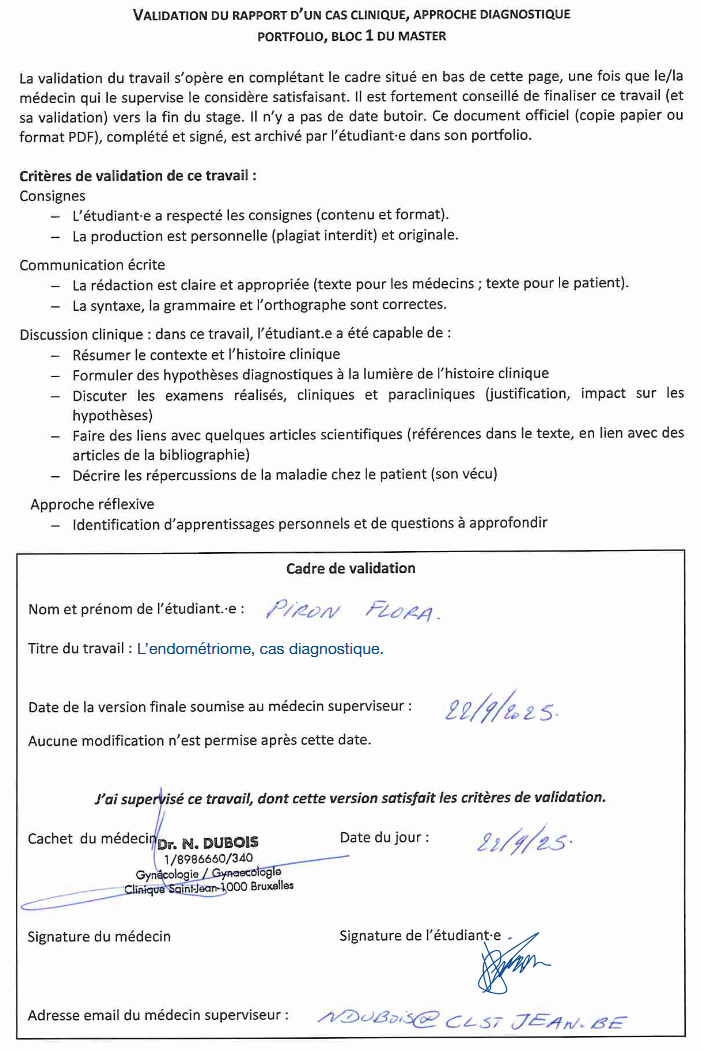
\includegraphics[width=0.9\textwidth]{images/cas_diagnostique/fiche_validation_DrDuboisV2.png}
    \caption{fiche validation}
    \label{fig:fiche_validation_DrDubois}
\end{figure}
\geometrieWord

\geometrieLarge
\begin{titlepage}

\begin{center}
\vspace*{.06\textheight}
{\scshape\LARGE UCLouvain\par}\vspace{1.5cm} % University name
\textsc{\Large Bachelor Thesis}\\[0.5cm] % Thesis type

{\huge \bfseries Activité extérieure\par}\vspace{0.4cm} % Thesis title
 
\begin{minipage}[t]{0.4\textwidth}
\begin{flushleft} \large
\emph{Author:}\\
\theauthor % Author name - remove the \href bracket to remove the link
\end{flushleft}
\end{minipage}
\begin{minipage}[t]{0.4\textwidth}
\begin{flushright} \large
\emph{Supervisor:} \\
Dr. Pascaline Jacquemart % Supervisor name - remove the \href bracket to remove the link  
\end{flushright}
\end{minipage}\\[3cm]
 
 
\vfill
\end{center}
\end{titlepage}
\geometrieWord

\chapter{Activité extérieure}
Spectacle de danse : Yé ! (L’Eau), par Circus Baobab, 23 novembre 2024 à la Maison de la culture d’Arlon. 
Dr. P. Jacquemart

\section{Résumé et justification de l'activité}

\todoH{FloraStyle}{red!30}{\ les corps du spectacle  sont différents par rapport à l’europe (choix pe des gens plus filiformes dans les compagnies europiénnes) pe ajouter une ligne sur ce thème}{}

L’activité culturelle que je souhaite détailler est un spectacle de \todoH{FloraStyle}{red!30}{\ est-ce que c'est la bonne façon de citer ou i faut mettre en textcite ?? }{danse, Yé ! (L’Eau)} \parencite{circusbaobab_site}. La danse est un moyen de communication unique soumis l’interprétation de chacun. Cet art requiert une certaine sensibilité et imagination afin d’en comprendre toute son histoire. Apprendre à voir au-delà, comprendre un message au travers des lignes du corps au lieu de celles des livres. La danse est un moyen d’ouvrir l’esprit afin de mieux comprendre l’autre. Tout le monde n’a pas le même langage et pourtant en suivant la gestuelle de la danse, une union se fait entre les spectateurs et les danseurs.  Ayant moi-même pratiqué la danse, je ne pouvais qu’admirer tous ces corps se mouvant à l'unisson. Poids plume, les danseurs étaient impressionnants et au-delà de la prouesse physique, ils ont, selon moi, su transmettre un message fort.
 
Yé ! représente avec force la question de nos ressources actuelles, et leur absence cruelle dans certaines régions du monde. Les danseurs se battent pour atteindre cette eau inaccessible. Ils représentent les Hommes qui se réinventent, construisent mais se déconstruisent également entre eux au nom de la santé, de la vie. Ces voltigeurs créent de véritables pyramides humaines aussi fortes que fragiles grâce à un équilibre étroit. A travers ce spectacle, les danseurs tentent de nous transporter et de nous transmettre l’espoir d’un avenir meilleur. Si, ensemble, nous agissons malgré une situation actuelle plus qu’alarmante. La thématique environnementale était rythmée par la friction des bouteilles en plastique, symboles percutants de la crise climatique actuelle et le fardeau de nos déchets. En effet, le décor était plus que minimaliste, un tapis de bouteilles était l’unique accessoire des danseurs. Loin d’un ballet classique, le contemporain permet une plus grande liberté d’expression et de mouvements. Une empreinte circassienne a également imprégné cette performance.
 
L’un des points de vue inspirants de ce spectacle est la place qu’il accorde à ses danseurs en tant qu’individus et artistes. En effet, le Circus Baobab est une troupe de cirque itinérante. Il a vu le jour en Guinée grâce à Laurent Chevallier, un célèbre réalisateur de cinéma. La compagnie permet à de nombreux danseurs d’avoir un métier stable et de sortir de la précarité. Alors que leur tournée ne s’étendait qu’aux villages environnants, de nos jours, ils traversent toute la France et ses pays limitrophes pour s’exprimer et faire voyager les spectateurs à travers la danse. Ils utilisent les réseaux sociaux pour faire connaître leur cause. Ils n’hésitent pas à montrer leur engagement auprès des plus jeunes car ils recrutent régulièrement. Ils publient également les heures d’entraînement passées afin de nous faire vivre une expérience hors norme ainsi que leur succès et toutes les différentes populations qu’ils ont réussi à toucher avec leurs messages. En outre, ces représentations révèlent des silhouettes rarement observées au sein des compagnies européennes, elles constituent ainsi une invitation à la tolérance et à l'acceptation de la pluralité des corps.

Lorsque le rideau tombe, une réflexion naît. Une fois de plus c’est un rappel de la chance que nous avons dans notre pays, les ressources et le système de santé aussi développés tout en ajoutant une touche de culpabilité car si d’autres régions sont moins chanceuses, des actions peuvent être faites chez nous pour changer les choses. Avoir un rappel aussi délicat et artistique permet d’écouter le message sans se sentir impuissant. De plus, sachant l’histoire de la compagnie, se dire qu’en regardant simplement un spectacle nous rendons possibles à ces danseurs de continuer leur route et de soutenir leurs actions. Ce spectacle ne demande qu’à être regardé, écouté et à ouvrir la porte à la réflexion.

En dehors du cadre académique, je suis convaincue qu’il est primordial d’être ouvert à d’autres façons d’apprendre et de voir le monde. Spécialement dans notre médecine actuelle qui fait face à bien plus de \todoH{FloraStyle}{red!30}{\ défis ? lesquels frustrations de pas les détailler, changer la formulation pour fermer les propositions  }{défis} que les soins du patient. Parmi ces défis, je peux notamment citer l'élaboration particulière de la relation patient-médecin ou encore la conscience de la santé planétaire ou même les aspects économiques des soins.
\section{Impact sur ma pratique future}

Bien que la connaissance factuelle et la rigueur soient des fondements essentiels de la pratique médicale, compte tenu des enjeux vitaux, il serait réducteur de s'arrêter là. Ne risquons-nous pas de perdre l'essence de la relation humaine si nous échouons à décoder ce qui se transmet au-delà du verbal ? Le langage non-verbal est, en effet, aussi un vecteur fondamental de la communication médecin-patient. À cet égard, la célèbre théorie d'Albert Mehrabian \parencite{demetersante2022}, qui attribue une part prépondérante au non-verbal ($55$\% pour le langage corporel) dans la communication des attitudes et des émotions, confirme l'impératif de développer cette compétence. Apprendre à interpréter les signaux corporels du patient devient alors une composante nécéssaire à notre formation. Ce besoin est amplifié face aux patients dont l'expression est limitée par des facteurs tels que l'âge, la langue, la culture ou la pathologie. La danse, en tant qu'expression corporelle par excellence, représente ainsi une éducation précieuse à l'observation fine de l'autre.\\

\todoH{FloraStyle}{red!30}{\ passage trop stigmatisant. MG médecine environnementale !!! apporter des nuances }{\mbox{Au-delà de l'émotion artistique}}, cette expérience invite à explorer le concept du One Health défini par une approche systémique reconnaissant que la santé humaine, la santé animale et l'équilibre des écosystèmes sont fondamentalement interdépendants. L’antibiorésistance illustre parfaitement la nécessité de cette approche. Face à cette menace, les mesures traditionnelles de la médecine humaine (contrôle des prescriptions, recherche, hygiène hospitalière) restent insuffisantes. Le One Health impose une vision systémique et multidisciplinaire. Concrètement, cela implique d'optimiser les prescriptions médicales et vétérinaires, mais aussi d'améliorer le traitement des \todoH{FloraStyle}{red!30}{\ perturbateurs endocriniens dans les eaux usées pas que AB --> il y a plein d'exemples possibles mais questions de nombre de mots, je ne vais pas en parler}{eaux usées} pour y réduire la concentration d’antibiotiques et de bactéries résistantes. L'éducation et la prévention auprès de tous ces professionnels (soignants, vétérinaires, agriculteurs) sont également primordiales. Heureusement, des transitions s'opèrent déjà dans l'enseignement professionnel : en Belgique, l'utilisation des huiles essentielles \parencite{siep_formation_524} en agronomie est enseignée comme alternative aux antibiotiques en élevage, avec des plans d'actions aux résultats encourageants selon \textcite{celagri_antibioresistance}.\\
Je suis convaincue que l’intégration du One Health représente l’avenir d'une médecine engagée et préventive, vers laquelle notre formation tend de plus en plus. À notre échelle, des gestes cliniques modestes (une anamnèse approfondie, un examen rigoureux et une prescription réfléchie avant tout examen complémentaire) contribuent déjà à une pratique plus durable et à la transformation globale de notre manière de soigner.\\


Certes, cette vision peut sembler idéaliste, mais elle est porteuse d’espoir. Même si cette transition vers une médecine plus responsable ne se fera pas en un jour, elle se fera. Ce "micro-rappel" précieux nous recentre sur l’essentiel et nous ouvre à une réflexion plus large sur notre mission de soignant.
\section{Conclusion}

Vous présenter un spectacle de danse rappelle que soigner, c’est avant tout écouter sans parole et accueillir sans jugement. J’ai été profondément touchée par l'engagement de cette troupe modeste, qui porte un message fort tout en transformant concrètement l'avenir de ses jeunes danseurs. En ajoutant la thématique du OneHealth qui est un sujet incontournable dans notre médecine moderne et l’aborder à travers la danse est une idée qui me correspond. Cette perspective globale du soin, à la fois intime et planétaire, est une conviction que je souhaite garder tout au long de ma formation et de ma pratique future.

\chapter{Cas thérapeutique}
\section{Résumé du cas clinique}

\subsection{Motif}
La patiente se présente aux urgences, le $30$ décembre $2025$, accompagnée de la police pour une demande d’internement à la suite d'une tentative de suicide.

\subsection{Contexte social}
La patiente a $60$ ans, elle a un fils de $27$ ans. Elle s’est séparée du père lorsque celle-ci était encore enceinte. Depuis madame vit seule avec son fils.

Au niveau professionnel, elle est pensionnée depuis le $1$ janvier $2026$. Elle a fait carrière en tant que secrétaire de direction.

La patiente rapporte avoir été victime de violence dans son enfance. 
Ensuite, son ancien compagnon était violent avec elle. De plus, l’enfant est issu d’un viol de celui-ci. Elle a toutefois, décidé de se séparer de cet homme tout en gardant l’enfant et en l’élevant en tant que mère célibataire. Actuellement elle subit des violences physiques et verbales de la part de son fils rendant la situation intenable au domicile. Celui-ci a été diagnostiqué dès son plus jeune âge de trouble de l’attention et d’hyperactivité ainsi que du trouble du spectre autistique. En effet, il présente un comportement violant à la moindre contrariété. Celui-ci a un suivi psychiatrique mais n’a pas de situation professionnelle ni logement.

\subsection{Antécédents psychiatriques}
\begin{itemize}[label=\textbullet]
    \item \underLine{Depuis l’âge de $18$ ans} : dépression récurrente.
    \item  \underLine{De $2015$ à $2021$ } : suivi psychiatrique mais aucun suivi ambulatoire depuis.
    \item \underLine{ $2021$} : dépendance aux benzodiazépines.
    \item \underLine{ $2021$ et juillet $2025$} : $2$ hospitalisations pour dépression.
\end{itemize}

\subsection{Antécédents somatiques}
\begin{itemize}[label=\textbullet]
    \item Actuellement en rémission d’un mélanome.
    \item Thyroïdite d’Hashimoto  
    \item Fibromyalgie
    \item Vessie hypertonique
    \item Diarrhées chroniques idiopathiques
\end{itemize}

\subsection{Allergies}
\begin{itemize}[label=\textbullet]
    \item Moxifloxacine 
\end{itemize}
 
\subsection{Antécédents familiaux}
\begin{itemize}[label=\textbullet]
    \item Son père affecté d’un cancer prostatique au stade métastatique. 
\end{itemize}

\subsection{Anamnèse}  
Suite à une tentative d’étranglement de la part de son fils, la patiente aurait fait une tentative de suicide. La patiente dit avoir pris $5-6$ comprimés de lormétazépam $2$mg, $6-7$comprimés de lorazépam $1$mg, $2$ comprimés d'alprazolam retard dont la dose est inconnue. Elle aurait été retrouvée inconsciente à l’arrivée de la Police qui avait été prévenue par les voisins. Elle souhaite inscrire son fils auprès d’associations qui pourraient l’aider à trouver un logement et un travail mais les délais d’attente sont longs. La patiente ne voit pas de solutions possibles à court terme. Malgré la thymie triste et les ruminations suicidaires qui persistent, la patiente se projette dans l’avenir et a des projets. 

\subsection{Examen clinique}
La patiente est anxieuse avec une thymie triste et labile.
Elle est cohérente. Une hypoprosexie est observée. 
Son discours est volubile et circonlocutoire pouvant témoigner d’une grande charge anxieuse associé à des difficultés d’attention et une accélération psychique. 
La patient présente des insomnies de maintien. 
Sur le plan psycho-affectif, on note une intense ambivalence vis-à-vis du fils. 
La patiente oscille entre un désir de protection maternelle, teinté de culpabilité, et un besoin de mise à distance vitale face aux hétéro-agressions subies. Cette dynamique relationnelle complexe alimente un sentiment d'impasse existentielle, majorant le risque suicidaire. 
Une hyper-émotivité est observée chez la patiente ce qui se perçoit comme une personne qui s’implique beaucoup avec les personnes qui sont bienveillantes avec elle. 

\subsection{Examens complémentaires}
\begin{itemize}[label=\textbullet]
    \item Biologie : sans particularité mis à part une hypercholestérolémie à $243$mg/dl. (Ionogramme et fonction rénale (>$60$ mL/min) sont corrects).
    \item ECG : rythme sinusal, FC $80$bpm
\end{itemize}
Voir détails des examens complémentaires en \cref{annexe:examens_complementaires} en \cpageref{annexe:examens_complementaires}.

\subsection{Diagnostic retenu}
 
Épisode dépressif majeur avec caractéristiques mixtes\footnote{\url{https://www.infodrog.ch/files/content/refbases/DSM-5_Manuel-diagnostique-et-statistique-des-troubles-mentaux.pdf\#page=286} \parencite{dsm5_online}}  dans un contexte familial relationnel difficile.

\subsection{Traitements réalisés et prise en charge} 
\begin{itemize}[label=\textbullet]
    \item Paroxétine (Seroxat)  $20$mg $1$cp/j
    \item Zopiclone (Imovane) $7,5$mg $1$cp/j
    \item Olanzapine (Zyprexa) $5$mg $1$cp/j 
    \item Lorazépam (Temesta) $2,5$mg $1$cp/j
    \item Lévothyroxine sodique (T4, 100 µg) et liothyronine sodique (T3, 20 µg) (Euthyral) $75$mg $1$cp/j 
    \item Lopéramide (Imodium) $2$mg $2$cp/j
    \item Fésotérodine (Toviaz) $4$mg $1$cp/j 
\end{itemize}
 
Ce traitement pharmacologique est associé à une psychothérapie et l’hospitalisation sera suivi d’une cure psychothérapeutique stationnaire. 
Une assistante sociale s’intéresse également au cas afin de tenter d’apporter des solutions dans la sphère sociale de la patiente. 
 
Lors de l’hospitalisation, un changement au niveau du traitement a eu lieu. Le valproate de sodium $500$mg a été remplacé par l’olanzapine $5$mg principalement à cause d’une chute de cheveux marquée lors de l’augmentation de la posologie du valproate. De l’olanzapine est mis à la place avec effet positif thymorégulateur et nette atténuation des fluctuations émotionnelles au cours d’une même journée. 
 
L’abandon de la quétiapine $20$mg a également eu lieu car elle a présenté des éruptions cutanées. 

\subsection{Évolution de l’hospitalisation }
Amélioration thymique et amélioration de son sommeil. 
La patiente a des idées noires passagères toutefois dans l’évolution de son hospitalisation, celle-ci demande de l’aide auprès des soignants. 
La patiente apprend a posé ses limites auprès de son entourage. 

\subsection{Ressenti de la patiente}
La patiente semble être demandeuse de traitement et a une volonté d’aller mieux. La patiente voit son hospitalisation comme un moyen se protéger de son fils et comme une ressource sociale pour l’aider dans les démarches administratives et trouver des solutions.
 
Concernant son traitement psychiatrique, la patiente associe cela à un même besoin qu’un traitement somatique. Elle a toujours considéré sa santé mentale au même titre que sa santé physique. Il est donc normal pour elle de prendre un traitement quotidiennement. 
La patiente se décrit comme une personne «hypersensible» pharmacologiquement parlant, en d’autres termes, avec le temps, elle a eu l’occasion de tester de nombreuses molécules différentes et selon elle, elle ressentirait les effets secondaires plus fréquemment que la population générale et avec des doses plus faibles. Au cours de sa prise en charge avec son psychiatre extérieur, elle dit n’avoir jamais trouvé l’équilibre entre bénéfices et effets secondaires, y compris avec le valproate. Depuis l’instauration de l’olanzapine, elle se sent mieux. 
\section{Démarche de médecine factuelle}

\subsection{Informations scientifiques}
  
\subsubsection{Méthode}

PICO :
\begin{itemize}[label=\textbullet]
    \item Population : Patient souffrant d’un épisode dépressif résistant avec caractéristiques mixtes. 
    \item Intervention : l’ajout d’antipsychotiques au traitement antidépresseur. 
    \item Comparateur : placebo. 
    \item Outcome : obtenir une rémission des symptômes et prévenir les effets secondaires. 
\end{itemize}

Banque de données consultée : Pub Med.\\ 
Termes MeSH utilisés : «Major Depressive Disorder », «Mania» et «Antipsychotic Agents».\\
Critère pour la sélection d’article : publication dans les $5$ ans, «Free full text», «Randomized controlled trial», «Meta-analyse» et «Systematic review».\\
Date de consultation et nombre d’articles : le $07$ février $2026$, $2$ articles répondaient à ces critères. 

\subsubsection{Résultats}  

L'article choisi est le suivant, \textcite{gao2025efficacy}.
 
Les auteurs constatent une amélioration des symptômes dépressifs et maniaques avec les antipsychotiques chez les patients souffrant de MDE-MFS -- major depressive episodes with mixed features specifier. Ce traitement aurait un profil des effets secondaires bénéfiques sans risque augmenté d’effets secondaires sévères. Les stabilisateurs de l’humeur et certains antidépresseurs -- trazodone -- montreraient également une efficacité chez ces mêmes patients. Toutefois, la preuve de leur efficacité et leur sécurité étaient limitées et controversées dû au nombre restreint d’études disponibles.

\begin{figure}[H]
    \centering
    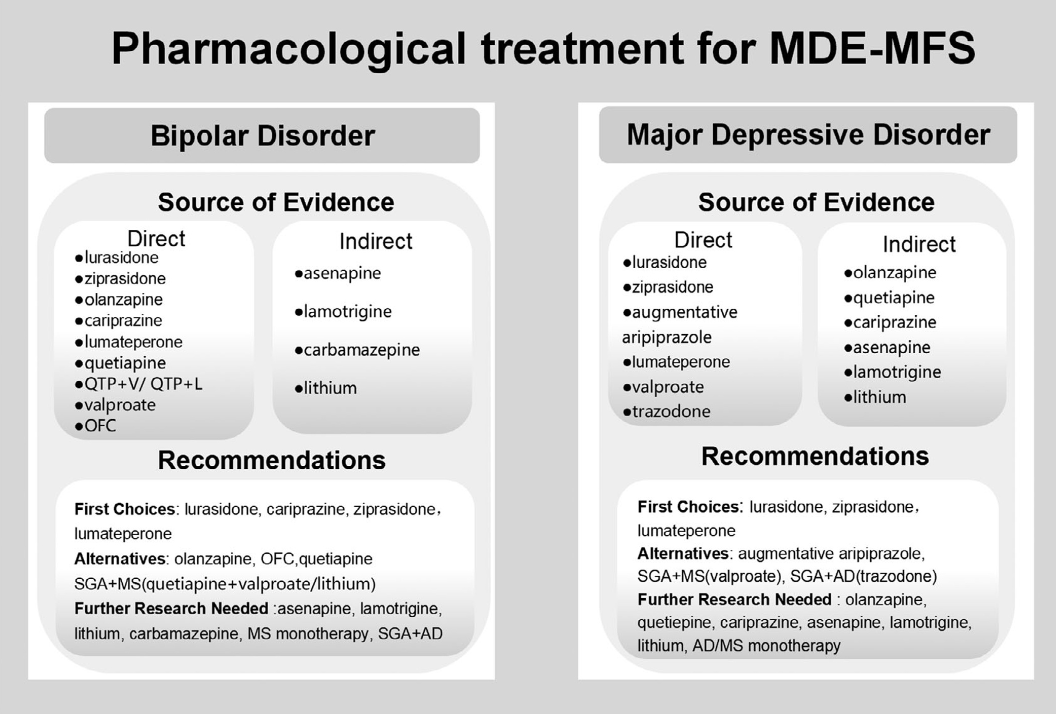
\includegraphics[width=\textwidth]{images/cas_therapeutique/resultat_etude_casM2.png}
    \caption{traitement pharmacologique pour MDE-MFS}
    \label{fig:resultat_etude_casM2}
\end{figure}

\subsubsection{Discussion}





\begin{itemize}[label=\textbullet]
    \item \textbf{Analyse critique de la méthodologie}\\
    La méthodologie de cette méta-analyse, notamment pour évaluer puis stratifier les différents articles selon leur biais, semble complète et rigoureuse tout à fait en accord avec l’EBM. Pour chaque nature d’article, différents outils adaptés ont été employés \todoH{FloraStyle}{red!30}{Cochrane tool (Higgins et al., 2011) : C'est le standard mondial ("gold standard") pour évaluer les biais dans les essais contrôlés randomisés (RCT). Il analyse précisément la randomisation et l'insu.
    Newcastle-Ottawa Scale (NOS) : C'est l'outil de référence pour les études observationnelles et les analyses post-hoc.
    ROBINS (Risk of Bias In Non-randomized Studies) : C'est l'outil le plus robuste recommandé par la collaboration Cochrane pour les études d'intervention non randomisées.
    Outils JBI (Joanna Briggs Institute) : Ils sont reconnus internationalement pour l'évaluation rigoureuse des séries de cas et des rapports de cas.}{(Cochrane pour les RCTs, NOS pour les études observationnelles, ROBINS pour les études ouvertes).}
    
    Concernant le biais de publication, il a été mesuré selon plusieurs outils, à nouveau pour argumenter et valider au mieux les résultats. Le funnel plot est cependant difficilement interprétable vu le nombre d’études sélectionnées inférieur à 10 mais le test d’Edgar avec p≥$0,05$ confirme l’absence de biais de publication significatif.
    
    L’analyse de la sensibilité via la méthode «leave-one-out» a démontré qu’une étude en particulier, l'étude de Singh et al. ($2020$) sur les adolescents, déstabilisait les résultat concernant les symptômes maniaques et donc montre un I$^2$ élevé. Afin de résoudre cette forte hétérogénéité, cette étude a été exclue. 
    
    Les méthodes utilisées pour interpréter les résultats de cette méta-analyse semblent répondre à l’EBM. Toutefois, le talon d’Achille de cette étude est le nombre d’études disponibles et leur qualité intrinsèque, en effet la majorité des articles étaient des analyses post-hoc, c’est-à-dire, des analyses qui n’avaient pas pour objet la thématique de cette méta-analyse mais dont les données ont été recueillies. Les auteurs qualifient donc cette méta-analyse de préliminaire, nécessitant par la suite des RCT prospectifs. De plus, les variations de définition de dépression avec caractéristiques mixtes sont retrouvées dans la littérature médicale ce qui complique la réalisation de la méta-analyse et peut-être biaise la sélection des patients. 
    
    \item \textbf{L'interprétation des principaux résultats}\\
    Concernant les antipsychotiques, le taux de réponse clinique est meilleur par rapport au placebo  (RR = $1.46$ [$95$\% CI: $1.31, 1.61$], p < $0.001$; NNT = $7 [95$\% CI: $5, 9$]).  Les autres outcomes primaires tels que l’évolution du \todoH{FloraStyle}{red!30}{\url{https://www.ciusss-capitalenationale.gouv.qc.ca/sites/d8/files/docs/ProfSante/Infirmier/evaluation-manie-young.pdf}}{score YMRS}, l’échelle d’évaluation de la manie de Young, montrent une nette réduction comparée au placebo (SMD = $0.35 [95\% CI: 0.53, 0.17], p < 0.001$). 
    
    Quant à l’outcome primaire de sécurité, TEM rate qui signifie le virage maniaque, n’est pas significativement différent du groupe contrôle (RR = $0.91 [95\% CI: 0.53, 1.55], p = 0.65$). Par contre, les antipsychotiques ont été associés à une recrudescence du risque d’effets secondairess classique par rapport au placebo (RR = $2.33 [95\% CI: 1.63,3.34], p < 0.001; NNH = 17 [95\% CI: 11,25$]) particulièrement pour les symptômes extrapyramidaux et le trouble de la vigilance et du sommeil.
    
    Les auteurs ont également analysé l’efficacité et la sécurité de différents types d’antipsychotiques chez les patients souffrant de d’épisodes dépressifs majeurs avec caractéristiques mixtes dans un contexte de dépression majeure. Cependant, le nombre restreint d'études disponibles pour ce profil clinique spécifique a limité les conclusions à une analyse descriptive, empêchant la réalisation d'une synthèse quantitative formelle. Malgré cette limite, les données révèlent une efficacité supérieure des antipsychotiques sur le placebo pour stabiliser les deux pôles de la pathologie. La lurasidone a notamment montré un taux de réponse supérieur au placebo ($64.8\% $versus $30.0\%, p < 0.001$), avec une amélioration des symptômes maniaques confirmée à long terme.  Sur le plan de la sécurité, aucune augmentation significative du risque de virage maniaque (taux de TEM) ou de symptômes extrapyramidaux (EPS) n'a été observée par rapport au placebo, les effets indésirables courants comme la somnolence ou les nausées restant généralement modérés et tolérables.
    
    Toujours en reprenant cette population précise, une étude a montré une amélioration significative des symptômes dépressifs grâce aux stabilisateurs de l’humeur (valproate) à dose moyenne chez $18/22$ patients. Lors du suivi, certains ont rapporté des effets secondaires et un tiers de ces personnes ont arrêté le traitement pour cette raison. Deux études rétrospectives indiquent enfin que la trazodone pourrait réduire efficacement l’agitation et les symptômes mixtes avec un profil de sécurité rassurant, bien que l’absence de groupe contrôle impose de considérer ces résultats comme préliminaires.
\end{itemize}
 
\subsubsection{Conclusion} 
 
Cet article confirme les guidelines et appuie la sécurité et l’efficacité des antipsychotiques, régulateur de l’humeur et de certains antidépresseurs dans ce contexte de MDD avec MDE-MFS. Toutefois, il faut garder à l’esprit les limites de cette méta-analyse notamment le nombre limité d’études disponibles et que les auteurs ont décidé d’inclure des analyses post-hoc. 
 
\subsection{Contextualisation}
La patiente, au cours de sa prise en charge, a souffert de nombreux effets secondaires. Certains s’associent à des pathologies déjà présentent, notamment les troubles de transites qui s’additionnent aux diarrhées chroniques idiopathiques. 

En pratique, vu les traitements antérieurs et leur tolérance chez la patiente, plusieurs molécules étaient éliminées dont la quétiapine, le valproate. Un régulateur de l’humeur était à envisager compte tenu des caractéristiques mixtes de sa dépression. L'olanzapine semblait donc une molécule de choix pour associé à la paroxetine vu son efficacité prouvée sur ce type de diagnostic. Cependant, l'hypercholestérolémie objectivée par le bilan biologique constitue un paramètre de vigilance majeur, car l'olanzapine est étroitement associée à un risque accru de dyslipidémie et de syndrome métabolique.

Si l’on suit les recommandations de la méta-analyse la lurasidone pourrait être également une alternative vu son profil d’efficacité et de tolérance dans la population MDD avec MDE-MFS. La trazodone pourrait également apporter des effets positifs chez la patiente, tout en s’assurant de la bonne tolérance de la patiente.

Il est important de noter que la patiente est compliante et vu son éducation thérapeutique et ses croyances, avoir un traitement comprenant plusieurs comprimés quotidiens ne représente pas un obstacle à la prise en charge.

La prise en charge de la patiente doit prendre en considération la sphère sociale. En particulier, le déclencheur principal de cette hospitalisation a été son fils. Par conséquence, la situation ne sera pas résolue tant que le fils habitera avec la patiente. C’est pourquoi une cure psychothérapeutique stationnaire a, en partie, été mise en place afin de solutionner temporairement le problème social et évidemment pour traiter la patiente au niveau psychologique. Le traitement médicamenteux a aussi son rôle à jouer pour stabiliser la patiente à court terme lorsque le travail psychologique et social se résout à long terme. 

\subsection{Intégration}
La littérature médicale permet de guider le praticien. Bien sûr les guidelines ont leur place dans la prise de décision du médecin. Cependant, la patiente doit être au centre des soins et elle n’est pas égale à la population générale. Il faut donc adapter sa prise en charge à la personne qui est souffre de la pathologie en question et l’adapter à son contexte social et familial. Dans ce cas, la patiente a besoin de prise en charge psychologique et sociale qui ne peuvent pas se résoudre rapidement. La décision d’un traitement médicamenteux est justifiée vu les effets bénéfiques sur les symptômes de la patiente.

Concernant le choix de la molécule, sa tolérance particulière aux molécules, marquée par une susceptibilité allergique cutanée, devient ici le principal guide du choix thérapeutique, primant sur les recommandations générales de première intention ou celles avancées par la méta-analyse. De plus, en pratique, toutes les molécules ne sont pas disponibles au Grand-Duché du Luxembourg notamment lurasidone. Le praticien doit donc adapter sa prise en charge en fonction des limitations pratiques qui se présentent à lui.
\section{Approche réflexive}

\subsection{Si vous deviez ne retenir qu’une seule notion de ce travail, quelle serait-elle ?}
Si je ne devais retenir qu’une seule notion de ce travail, ce serait l’importance cruciale d’une approche holistique et centrée sur la personne lors de l’initiation d’un traitement. L’EBM ne se limite pas aux statistiques d’efficacité brute, elle doit intégrer les comorbidités et, surtout, le ressenti subjectif du patient. Considérer une plainte qui impacte le quotidien est le garant de l’alliance thérapeutique. Sans ce sentiment d’être écoutée, la compliance est menacée, particulièrement dans des pathologies instables comme la dépression mixte.

Cette vision rejoint la pensée d’Édouard Zarifian qui, dans La Force de guérir \parencite{zarifian1999force}, souligne que la pratique psychiatrique est indissociable du lien humain et du contexte culturel. Il nous rappelle que la prise en charge s'inscrit dans un cadre social large qui influence directement le regard des médecins et leurs processus diagnostiques. L'élimination du seul symptôme par la technique est insuffisante si l'on ignore le sens que le patient lui donne au sein de son histoire personnelle.

\subsection{Que pensez-vous avoir bien réussi dans ce travail ?}
Le rapport de cas a été un exercice fréquent lors de mon stage, à travers celui-ci j’ai tenté de m’améliorer au mieux. Concrètement, j'ai tenté de décrire un tableau global tout en insistant sur les éléments pertinents. La patiente a vécu beaucoup d’expériences parfois traumatisantes dans sa vie. Plusieurs interprétations peuvent être faites sur l’évolution de la patiente et sur les raisons de son hospitalisation. Grâce à la collaboration étroite avec les psychiatres présents dans le service, j’ai pu communiquer mes pensées et démarches cliniques afin qu’ils puissent me guider et me corriger si nécessaire. Il y également eu un apprentissage constant pour réaliser une transmission claire et des hypothèses construites. 

\subsection{Que pensez-vous devoir améliorer ?}
J’ai tenté de maîtriser la recherche sur différentes bases de données au mieux mais je ressens un manque d’expérience particulièrement pour le choix des MESH-Terms. L’interprétation de chaque donnée individuelle a été, selon moi, bien comprise et réalisée mais mon assurance diminue quand la décision finale de la fiabilité de l’article n’est pas évidente et reste nuancée. J'ai tenté de m’appuyer sur des éléments objectifs afin d’aiguiser mon opinion.  

\subsection{Quelle(s) question(s) souhaiteriez-vous approfondir dans un prochain travail ?}
Je pense qu’aborder le suivi plus long terme de la patiente et son évolution dans le temps aurait pu être très intéressant. En outre, la démarche sociale et psychologique aurait pu être davantage approfondie et mise en avant. Effectivement, je suis convaincue que la prise en charge doit être multidisciplinaire et que l’aspect purement médicamenteux de cette prise en charge est nécessaire mais loin d'être suffisante et la place de la psychothérapie a une place déterminante dans l’évolution de l’état psychique de la patiente. Je pense que se renseigner sur les différents types de psychothérapie -- leur durée, les effets de la communication sur la patiente -- est primordial à maîtriser. Sans doute, dans notre médecine actuelle, le focus est peut-être trop axé sur la pharmacologie. 
\geometrieLarge
\begin{figure}
    \centering
    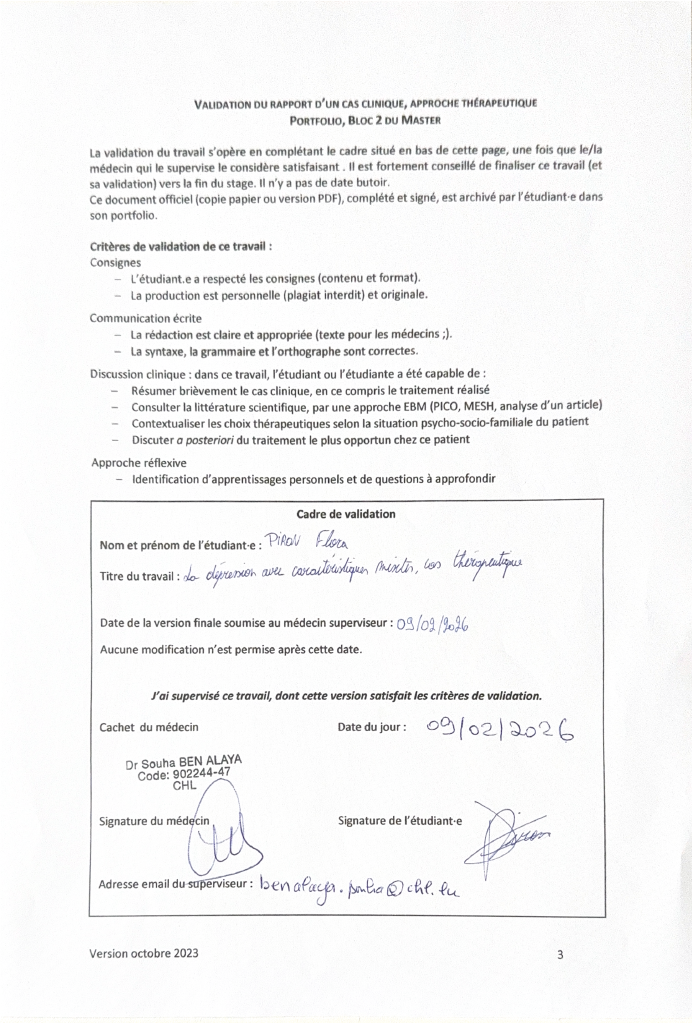
\includegraphics[width=0.9\textwidth]{images/cas_therapeutique/Fiche_Validation_casM2.png}
    \caption{fiche validation}
    \label{fig:fiche_validation_DrBenAlaya}
\end{figure}
\geometrieWord

\chapter{Incident médical}
\section{Description de l'incident}

Un patient est né dans un contexte de déni de grossesse jusqu’à l’accouchement dans un hôpital à $40$SA. En effet, la maman en devenir s’est présentée aux urgences pour maux de dos. Suite à cela, l’accouchement a eu lieu. Retour à domicile du patient et de sa famille tel un accouchement classique au bout de $4$ jours, sans procédure supplémentaire.\\ 

Dans le cadre de son suivi pédiatrique, l’enfant a été vu pour son vaccin des $2$ mois. A ce moment, une hypotonie et une perte de poids importante sont mises en évidence : poids de naissance est de $4,060$kg, lors du premier mois de vie, il y a une prise de $50$g puis une perte de $500$g. Une hospitalisation aux soins intensifs est mise en place. A la sortie des soins intensifs 16 jours plus tard, l’enfant pèse $4,545$kg. En parallèle, une évaluation sociale est en cours car une dénutrition par manque d’apport est évoquée. Ensuite, l’enfant est transféré et poursuit son hospitalisation durant $48$h vu la bonne prise de poids observée. De plus, l’équipe médicale s’intéresse au contexte familial au sens large car le patient a une fratrie, nous tentons donc d’assurer la bonne santé de ces enfants. Un signalement pour la protection de l’enfant est considéré mais n’est pas appliqué. Selon l’équipe multidisciplinaire, une chance supplémentaire est donnée à ces parents vu le contexte de déni de grossesse et un deuil du côté maternel qui s’est additionné à la situation sociale lors du premier mois de vie du patient. Des aides dans le quotidien de cette famille et un suivi rapproché sont également mis en place.\\

Deux semaines plus tard, une consultation post-hospitalisation est programmée. A nouveau une perte de poids est observée. L’enfant est à nouveau hospitalisé pour dénutrition sévère. Une fois l’alimentation recontrôlée par les soignants, l’enfant reprend du poids. En outre, lors de l’hospitalisation, aucun lien d’attachement n’est observé entre la maman et le patient. La maman ne porte que peu d’attention à celui-ci et elle garde une expression neutre tout au long de l’hospitalisation même lorsque nous évoquons la gravité de la situation. Un signalement pour protection de l’enfance est mis en place et approuvé par la Juge responsable du cas. S’en suit le retrait de la garde de l’enfant par la Police.\\

L’enfant poursuit donc son hospitalisation sous la garde de l’hôpital et une prise de poids est toujours observée. Les parents expriment de l’incompréhension et défendent qu’ils prennent soin de leur enfant attribuant la perte de poids sévère à la présence d’adénovirus dans les selles du patient. Or, l’équipe médicale est formelle que celui-ci ne peut être responsable à lui seul de cette chute de poids drastique. Cependant, un bilan complémentaire afin d’exclure tout autre diagnostic pouvant expliquer la situation est en cours. L’avenir de cet enfant reste incertain à ce jour, sera-t-il placé en foyer ou en famille d’accueil ? Aura-t-il encore des contacts avec ses parents ? Son état général et son hypotonie vont-ils se résoudre ? Qu’en deviendra-t-il de la fratrie ? Un suivi psychologique/ psychiatrique sera-t-il organisé pour la maman ? \\

\section{Implications éthiques, déontologiques et légales de l’incident }

La problématique qui m’interpelle d’emblée est le manque de prise en charge lors de la naissance de l’enfant. Suivre le protocole de naissance classique ne me semble pas adapté à la situation. La physiopathologie du déni de grossesse n’est pas encore élucidée entièrement à ce jour mais il est bien connu qu’il est le reflet d’un traumatisme chez la maman. De plus, le déni de grossesse total, c’est-à-dire jusqu’à l’accouchement, représente un facteur de risque du passage à l’acte et la maltraitance de l’enfant. L’accouchement est un bouleversement psychologique intense pour la maman. Elle se présente aux urgences, dans ce cas pour des lombalgies puis se retrouve engagée dans un travail  en vue d’une naissance. L’enfant n’est pas attendu, aucune relation n’a été créée lors de la grossesse, la femme n’a pas eu l’occasion de devenir mère comme l’explique Sophie Marinopoulos dans \textcite{marinopoulos_deni_2019}. A la naissance du patient, il y a un manquement clair au niveau de plusieurs principes de la Bioéthique selon Beauchamp et Childress. D’une part la bienfaisance vis-à-vis de l’enfant a été négligée vu les facteurs de risque de négligence et la prévention d’un point de vue médical qui était possible. D’autre part, la bienfaisance vis-à-vis de la mère. Le déni de grossesse montrant clairement une souffrance psychique qui aurait dû être explorée par un professionnel de santé formé.\\  

Une revue de la littérature,  \textcite{lagedamon2025accompagnement} appuie une fois de plus l’intérêt de prendre en charge la maman qui a souffert d’un déni de grossesse. Un protocole standardisé afin de prendre en charge le déni de grossesse manque cruellement ce qui a pour conséquence des prises en charge hétérogènes voire inexistantes. Or, un suivi psychologique pour la maman qui a un risque augmenté de stress post-traumatique ou dépression post partum, a montré des bénéfices. Les psychothérapies telles que EMDR, \textit{Eye Movement Desensitization and Reprocessing}, peuvent permettre une amélioration clinique de la maman. Ensuite, l’établissement d’un lien d’attachement avec son enfant est envisageable et peut permettre de prévenir les situations de négligence voire les néonaticides qui sont certes rares mais extrêmement graves.\\

Je remets également en question le respect du principe de la justice dans ce contexte. Autrement appelé l’équité, la justice consiste à traiter chaque personne de façon loyale, équitable et appropriée en fonction de ses spécificités. L’enfant a le droit d’avoir les mêmes chances de s’épanouir malgré un contexte de déni de grossesse et un milieu défavorisé. Est-il réellement éthique de ne pas avoir mis en place des aides autours de la famille afin de compenser l’environnement de l’enfant au moment de sa naissance ?\\

Je pourrais également ajouter à ce principe de justice comment peut-on demander à des parents ayant vécu un déni de grossesse total d’élever leur enfant comme une naissance classique sans outils, sans aide extérieure ?\\

Ce cas clinique met en lumière toute la complexité du signalement pour la protection de l’enfant dans un cadre de maltraitance. Le placement d’enfant soulève de nombreux défis éthiques. Le conflit entre la bienfaisance et la non-malfaisance est au centre du dilemme éthique. D’une part, la priorité est le bien-être de l’enfant voire la survie de celui-ci. Son passage en réanimation témoigne de l’urgence de la situation. La cassure de courbe de ce patient a été le point d’appel pour établir le diagnostic de malnutrition par manque d’apport. En effet, après la mise en évidence des facteurs de risque prédisposant à la maltraitance tel que l’état psychologique de la mère, le contexte de déni de grossesse, la situation financière de la famille, les connaissances des parents à propos du développement de l’enfant,…  les pédiatres responsables devaient évoquer la maltraitance comme expliqué dans ce clinical report \textcite{block2005failure}. De plus, la déontologie appuie d’autant plus le principe de bienfaisance. L’article 61 du code de Déontologie Médicale belge stipule que « \textit{Si la situation le justifie, et pour autant que la personne vulnérable capable de discernement y consente, le médecin s'adressera à un confrère compétent en la matière ou fera appel à une structure pluridisciplinaire spécifiquement établie pour gérer cette problématique. Si la personne vulnérable est menacée par un danger grave et imminent ou s'il y a des indices graves d'un danger sérieux et réel que d'autres personnes vulnérables soient victimes de maltraitance ou négligence et que le médecin n'a pas d'autre moyen d'offrir une protection, il peut avertir le procureur du Roi de ses constatations }». Suite à l’échec de la mise en place d’aide au domicile, une stratégie de non malfaisance dans le but de conserver la relation thérapeutique avec les parents, le signalement fut une solution envisageable pour l’ensemble de l’équipe médicale.\\

L’aspect légal intervient également dans la prise de décision du placement de l’enfant. La loi qui doit être prise en compte dans cette situation. Selon l'article $15, § 2$ de la loi du $22$ août $2002$ relative aux droits du patient, le médecin a le droit de déroger à la décision des parents (ou du représentant légal) si celle-ci met en danger la vie de l'enfant ou constitue une atteinte grave à sa santé. Donc, en considérant l’aspect légal, le corps médical a l’obligation de faire ce signalement dans l’immédiat afin d’assurer la survie du patient.\\ 

Toutefois, le principe de non-malfaisance doit être exploré dans cette situation. En effet, est-ce que le placement de l’enfant est la meilleure solution pour lui et son développement ? Il est démontré dans cette étude \textcite{poitras2017contacts} que le placement des jeunes enfants réduit la probabilité de réunification avec les parents biologiques et une stabilité de trajectoire. Selon eux, la stabilité de la trajectoire se définit par trois critères : les tentatives de réunification familiale, l’échec de la réunification et le nombre d’hébergements qu’a vécus l’enfant. Toutefois, plusieurs limites se retrouvent dans cette étude dont un échantillon de petite taille ce qui empêche de pouvoir interpréter les résultats avec certitude. Cependant, cette étude confirme également les résultats obtenus dans la littérature scientifique. Peut-on extrapoler cette instabilité de trajectoire comme représentation objective du malheur de l’enfant ou en tout cas d’une mauvaise prise en charge au final ?\\

Par contre, une autre étude, \textcite{mascaro2012evaluation} démontre l’importance d’apporter l’attention, la stimulation psychique et physique du nourrisson durant cette période critique. Sans cette attention, l’enfant peut développer un trouble important du développement d’où l’importance de sortir l’enfant de cet environnement négligent. La pouponnière peut être une option, si et seulement si elle peut assurer une prise en charge constante et régulière. Donc, la décision entre séparer l’enfant de sa famille et le placer dans une famille d’accueil ou une pouponnière est bien sûr à nuancer et comparer les soins qui sont possibles et à quelle fréquence concrètement ils peuvent être réalisés. Une autre remarque reprise dans cet article est l’importance de la persévérance. Celui-ci n’a effectué un suivi que sur 4 mois mais déjà dans ce délai, ils ont observé un rythme différent chez plusieurs enfants. Cela signifie donc, que le soignant responsable de l’enfant ne doit pas perdre espoir une fois les soins mis en place car des améliorations voire une reprise du développement physiologique est possible. Le dilemme éthique et la balance pour ou contre le placement de l’enfant n’est pas univoque, il s’agit d’un équilibre fragile.\\ 

En conclusion, le plus grand problème éthique que j’ai identifié dans cette situation clinique est le manque de prise en charge à la naissance du patient. Un autre aspect éthiquement intéressant est tout la complexité du placement de l’enfant pour sa survie et son bon développement ainsi que les alternatives de prises en charge possible pour l’enfant et le déni de grossesse de la maman.\\

\section{Conduite à tenir selon l’étudiante }

Différents scénarios sont envisageables mais selon moi, le scénario le plus éthique aurait été une prise en charge multidisciplinaire dès la naissance du patient et la découverte du déni de grossesse. Une prise en charge psychologique voire psychiatrique selon le contexte, me parait obligatoire pour prévenir toute maltraitance et trouble dans la relation mère-enfant ainsi que de désamorcer la culpabilité que la maman ressentira. Prolonger l’hospitalisation lors de la naissance jusqu’à observer un attachement entre l’enfant et la mère ou tout signe qui va en ce sens afin d’avoir l’assurance nécessaire pour permettre un retour à domicile me parais indispensable. La suite du plan thérapeutique comprendrait une mise en place des aides dans le quotidien de la famille et en plus, être attentif en tant que médecin au deuil que la maman a traversé lors des premières semaines de vie du patient. Je pense que cette prise en charge aurait pu prévenir le passage en réanimation. Sans même transformer trop les faits et idéaliser la psychothérapie, la surveillance extérieure de cette famille, avec un regard bienveillant et médical aurait permis de dépister la dénutrition plus précocement. Avec cette présence du monde médical, cela permet de gagner du temps et laisser l’opportunité d’aborder l’approche centrée sur le patient.\\ 

Apporter cependant une nuance à ce scénario utopique est primordial car la condition nécessaire pour que cela fonctionne est que les parents acceptent la prise en charge et la présence de l’équipe soignante dans leur quotidien. A nouveau, avec une approche centrée sur le patient, les soignants ne s’imposent pas aux patients donc je reste convaincue qu’avec une communication adaptée une relation thérapeutique peut être entretenue. Il est important de notifier également que les parents se sont présentés à plusieurs consultations médicales prévues ce qui montre une collaboration fragile mais présente. Sans doute, ceci est une porte d’entrée pour un travail ensemble dans l’intérêt du patient.\\

\todoH{FloraStyle}{red!30}{pe mettre ce lien en note bas de page parce que ça m'a inspiré pour trouver une conduite en plus à faire \url{https://www.yapaka.be/sites/yapaka.be/files/texte/15_06_19_le_deni_de_grossesse-a_mettre_en_ligne_0.pdf}}{Le professionnel de santé} a bien sûr son rôle à jouer dans la reconnaissance de la grossesse le plus tôt possible afin d’éviter un déni de grossesse total. Au-delà du diagnostic précoce qui permet de limiter les complications, il est simplement important que le médecin reconnaisse le phénomène et la déconstruction des croyances qui entourent le déni de grossesse. Éviter le tabou de celui-ci permet une meilleure prise en charge et éviter la dénutrition sévère par carence d’apport. Des protocoles standardisés pour encadrer la prise en charge du déni de grossesse permettent de limiter les erreurs individuelles de chaque médecin et d’uniformiser les connaissances. La rédaction de ces protocoles serait l’idéal et une des premières idées qui vient en tête. Toutefois, si je dois rester réaliste, je dois considérer la difficulté que cela représente de mener des études cliniques et pouvoir tirer des conclusions statistiquement significatives avec un échantillon aussi réduit et ainsi pouvoir élaborer des guidelines pertinentes.\\ 

Pour conclure ce cas clinique, je pense que la prise en charge réelle n’a pas été optimale et surtout aurait pu être différente à plusieurs niveaux. Cependant, je pense qu’il est toujours plus simple de réfléchir au cas clinique a posteriori, sans urgence et avec du recul sur l’évolution de la situation. La prise de décision est toujours influencée par de nombreux facteurs et parfois, certains arguments prennent plus de poids qu’ils ne devraient ce qui entraine des conséquences néfastes. Pour ce patient, la suite de son histoire a été tragique mais grâce à plusieurs garde-fous, l’enfant a survécu et l’espoir d’une amélioration de son développement est toujours possible.\\  

\section{Approche réflexive}
\subsection{Les connaissances/compétences acquises lors de la rédaction de cet incident clinique ;}
\begin{itemize}[label=\textbullet]
    \item Approfondir ma capacité de recherche dans la littérature car celle-ci était pauvre pour cette thématique. Rechercher de nouvelles bases de données et aiguiser d’autant plus mon esprit critique.
    \item La déconstruction sur certaines croyances vis-à-vis du déni de grossesse. J’ai eu l’occasion de développer la physiopathologie et d’améliorer la façon dont je souhaitais aborder les patientes expérimentant un déni. 
    \item Ce cas clinique a montré l’importance de la pluridisciplinarité. Au-delà de l’équipe soignante, il y avait une collaboration étroite avec l’assistante sociale et avec la Juge responsable. L’aspect social étant vraiment présent et imbriqué dans la santé et la clinique du patient que l’assistant social devient un membre primordial et fait partie intégrante de la prise en charge. 
    \item Observer de mes yeux l’absence de lien mère-enfant a provoqué en moi beaucoup d’émotions et d’incompréhension. Il m’a fallu apprendre à prendre du recul sur la situation et garder un professionnalisme sans laisser transparaître mes sentiments et moi-même me protéger de cet impact.
\end{itemize}

\subsection{Les influences probables de ce travail sur sa pratique médicale future ;}

\begin{itemize}[label=\textbullet]
    \item Ne pas stigmatiser les patients selon leur milieu social et prendre le temps de comprendre la problématique et le contexte. Celui-ci peut aider à la prise en charge et savoir comment communiquer et établir une relation de confiance avec le patient et sa famille.
    \item Préserver la curiosité d’en apprendre plus sur les pathologies que l’on rencontre en clinique. Se remettre en question sur les bases acquises et rester à jour au niveau du savoir médical.
\end{itemize}

\subsection{Les difficultés (dépendantes ou indépendantes de sa volonté) ayant entravé son acquisition de nouvelles connaissances/compétences au cours de cette expérience ;}

\begin{itemize}[label=\textbullet]
    \item La restriction de l’information contenue dans les protocoles ou rapport présent dans le dossier. Les anamnèses d’entrée sont clairement centrées sur la clinique, toutefois, vu le contexte, avoir davantage d’informations sur l’aspect social aurait été utile.
    \item En lien avec l’émotion ressentie, j’ai également ressenti beaucoup d’impuissance. Je pense qu’il est naturel d’avoir un réflexe correcteur face à ce patient si jeune qui subit beaucoup face à un environnement nuisible. Je peux ajouter que face au déni des parents, il était parfois difficile de trouver mes mots afin de rester professionnel et d’avoir les termes appropriés et juste dans le sens que e-je voulais leur donner.
\end{itemize}

\subsection{Les solutions que l’étudiant·e peut mettre en place pour remédier à ces difficultés.}

\begin{itemize}[label=\textbullet]
    \item Pour améliorer les rapports, je peux penser à ajouter de façon systématique un contexte social et détailler les circonstances d’admission. 
    \item Il est important de déconstruire ce réflexe qui parfois entrave la bonne prise en charge et la relation thérapeutique. Le premier pas est d’abord de le reconnaitre et d’en prendre conscience. Ensuite, si le besoin en est, communiquer de cette problématique à un collègue voire à un professionnel afin d’être accompagné dans cette démarche. Plusieurs ouvrages existent et aident le soignant qui prend la peine de les lire. 
    \item D’un point de vue purement communicationnel, je pense qu’il me reste beaucoup à apprendre et la formation peut-être multimodal via des cours, des ouvrages, des conférences,…
    \end{itemize}



%------------------------------------------------------------------------------------
%	FIN DU DOCUMENT
%------------------------------------------------------------------------------------
\appendix
\chapter{Examens complémentaires}
\label{annexe:examens_complementaires}
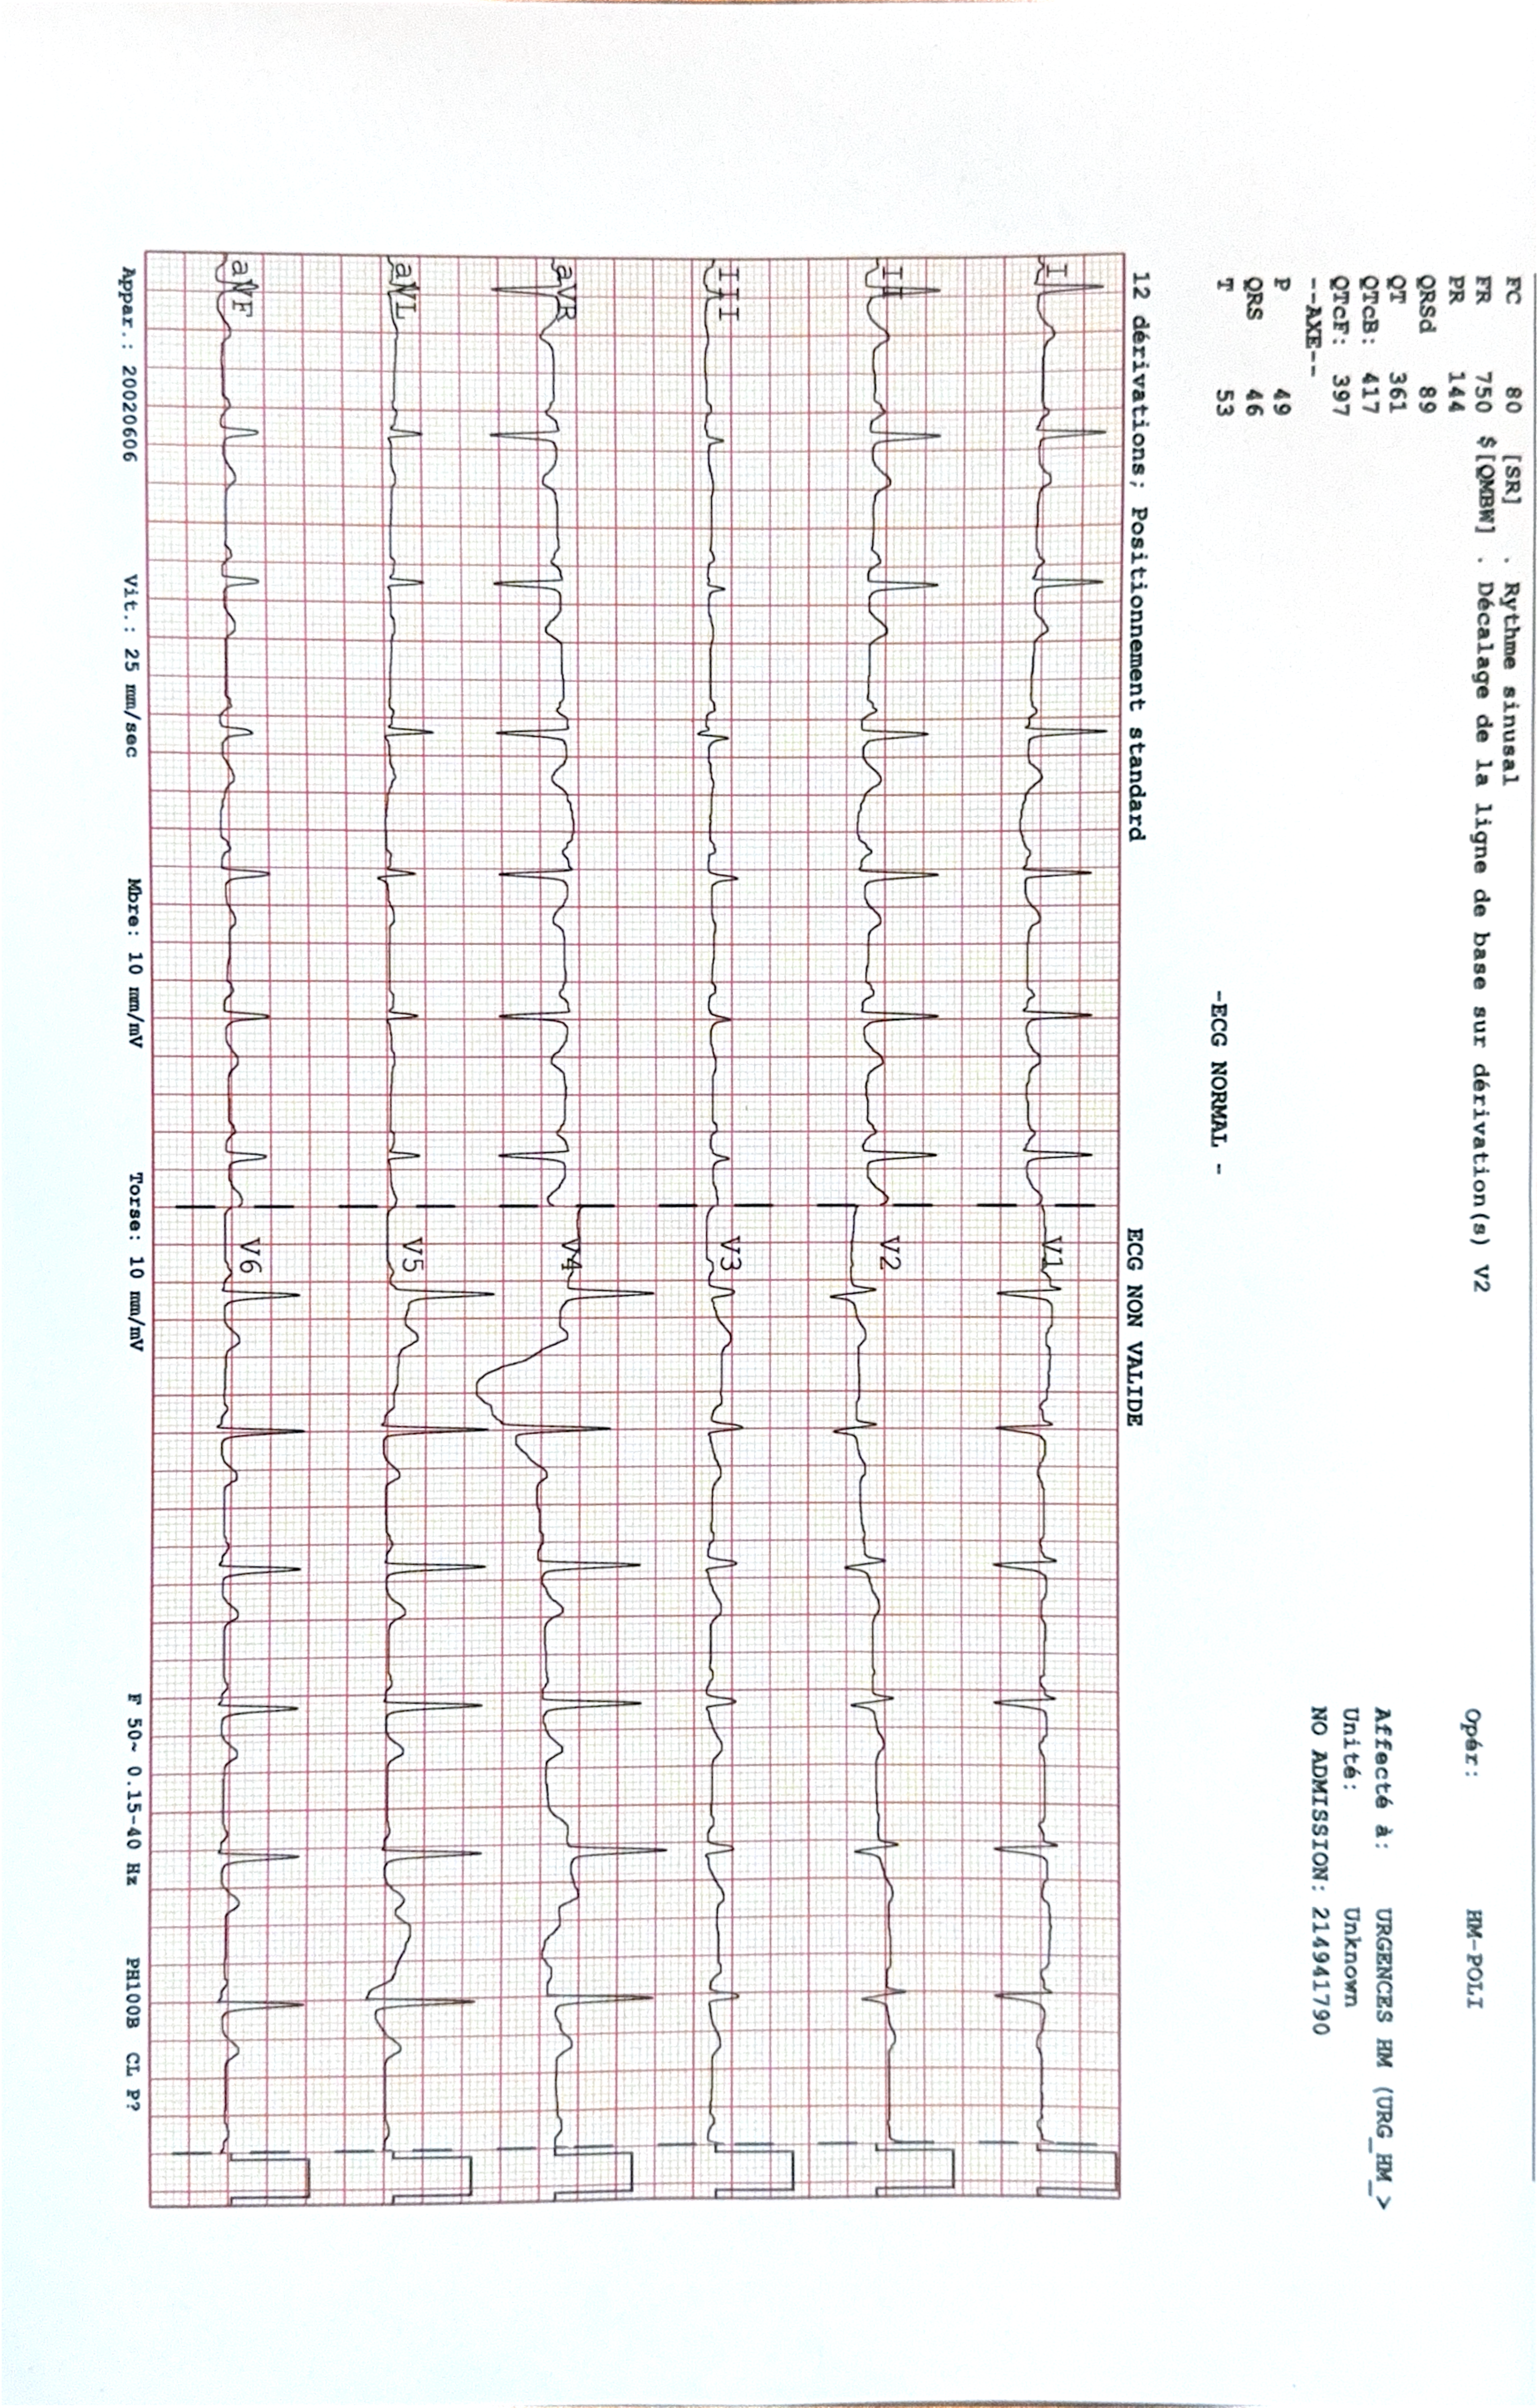
\includepdf[pages=-, pagecommand={\thispagestyle{plain}}]{images/cas_therapeutique/ExamenParacliniqueCasM2.pdf}

\backmatter
\listoffigures                              % Liste standard
\listofillustrations                        % Notre liste personnalisée
\listoftables
\printbibliography[title={Bibliographie}]

\end{document}